\documentclass[11pt]{article}

\usepackage[margin=1in]{geometry}
\usepackage{amsmath, amssymb}
\usepackage{siunitx}
\usepackage{graphicx}
\usepackage{hyperref}
\usepackage{tikz}
\usepackage{pgfplots}
\usepackage{enumitem}
\usepackage{parskip}
\usepackage{booktabs}
\usepackage{float}

\pgfplotsset{compat=1.18}

\title{APMA 2822B Homework 3 Report}
\author{Yash Agrawal}
\date{\today}

\begin{document}
\maketitle

\section*{Math Setup}
Assume that $\Delta x = \Delta y = h$. 

Using the second derivative approximations we were given, we have
\[
    f(x, y) = \frac{u[i-1, j] + u[i+1, j] + u[i, j-1] + u[i, j+1] - 4u[i, j]}{h^2}
\]

Substituting in the given $f(x, y)$, we get
\begin{align*}
    -8\pi^2 \sin(2\pi x) \cos(2\pi y) &= \frac{u[i-1, j] + u[i+1, j] + u[i, j-1] + u[i, j+1] - 4u[i, j]}{h^2} \\
    -8\pi^2 h^2 \sin(2\pi x) \cos(2\pi y) &= u[i-1, j] + u[i+1, j] + u[i, j-1] + u[i, j+1] - 4u[i, j]
\end{align*}

Solving for $u[i, j]$, we have
\begin{align*}
    4u[i, j] &= u[i-1, j] + u[i+1, j] + u[i, j-1] + u[i, j+1] + 8\pi^2 h^2 \sin(2\pi x) \cos(2\pi y) \\
    u[i, j] &= \frac{1}{4} \left( u[i-1, j] + u[i+1, j] + u[i, j-1] + u[i, j+1] + 8\pi^2 h^2 \sin(2\pi x) \cos(2\pi y) \right)
\end{align*}

We can use this equation to iteratively solve for $u$ with the given $f(x, y)$ using the Jacobi method. 

We will consider our solution to have converged when the maximum residual in $u$ across all grid points is less than a specified tolerance $\epsilon$. I chose $\epsilon = 0.001$ for this assignment.

\section*{Results}

I implemented three versions of the Jacobi iterative solver. One runs sequentially, one uses OpenMP to parallelize using shared memory, and one uses OpenMPI to parallelize using distributed memory. The OpenMP implementation uses 8 threads, and the OpenMPI implementation uses 8 processes. 

I also precompute the values of $f(x, y)$ and store them in an array to avoid recomputing them at every iteration. All my calculations will account for this precomputation in terms of the memory accesses and FLOPs.

All versions produce correct and also exactly identical results at every iteration. They converge when the max residual is less than 0.001. The performance results are summarized below, where N is the size of the array used.

\begin{table}[H]
    \centering
    \begin{tabular}{lrrrr}
        \toprule
        Version & N & Time (s) & GB/s & Iterations \\
        \midrule
        Sequential & 256 & 14.764 & 9.751 & 54,917 \\
        Sequential & 512 & 238.846 & 9.682 & 220,536 \\
        Sequential & 1024 & - & - & - \\
        OpenMP & 256 & 1.973 & 72.657 & 54,917 \\
        OpenMP & 512 & 24.469 & 95.506 & 220,536 \\
        OpenMP & 1024 & 375.660 & 98.686 & 883,877 \\
        OpenMPI & 256 & 2.340 & 61.519 & 54,917 \\
        OpenMPI & 512 & 37.489 & 61.685 & 220,536 \\
        OpenMPI & 1024 & 578.134 & 64.124 & 883,877 \\
        \bottomrule
    \end{tabular}
\end{table}

We can clearly observe that both of parallelism provided massive performance boosts. The OpenMP version performed better than the OpenMPI version by a significant margin. 

\section*{Roofline Model}

\subsection*{FLOPs}

To generate a roofline model, we first need to calculate the number of floating point operations (FLOPs) for our separate operations.

The FLOPs calculation depends on precomputing the values of $f(x, y)$ and storing them in an array.

For the loop in which we update our solution, we have the following operations for each grid point:
\begin{itemize}
    \item Scaling $f(x, y)$ by some constant: 1 FLOP
    \item Summing the four neighboring $u$ values: 3 FLOPs
    \item Adding the scaled $f(x, y)$ value to the sum of neighbors: 1 FLOP
    \item Dividing the total by 4: 1 FLOP
\end{itemize}

This gives a total of 6 FLOPs per grid point for updating our solution. Thus, the total number of FLOPs for updating our solution is \(6N^2\).

For the loop in which we calculate our max residual or convergence error, we have the following operations for each grid point:
\begin{itemize}
    \item Scale the current $u$ value by -4: 1 FLOP
    \item Sum the four neighboring $u$ values: 3 FLOPs
    \item Scale the resulting sum by \(1/h^2\): 1 FLOP
    \item Substract the result from the precomputed $f(x, y)$ value: 1 FLOP
\end{itemize}

While there are other operations, they are not floating point operations, so we do not count them here. This gives a total of 6 FLOPs per grid point for calculating the residual. Thus, the total number of FLOPs for calculating the residual is also \(6N^2\).

\subsection*{Memory Accesses}

We also need to calculate the memory usage for our separate operations. 

We use double precision floating point numbers for all calculations, which are each 8 bytes. Let the size of the matrix be $N \times N$.

For the loop in which we update our solution, we must read the u matrix, write the new u matrix, and read the f values matrix. This means the number of bytes we access for updating out matrix is
\[
    2 * 8 * N^2 + 8 * N^2 = 24N^2
\]

For the loop in which we calculate our max residual or convergence error, we must read the u matrix and the f values matrix. This gives the number of bytes accessed as
\[
    8 * N^2 + 8 * N^2 = 16N^2
\]

\subsection*{Arithmetic Intensity}

Using the FLOPs and memory access calculations above, we can calculate the arithmetic intensity for both operations.

We assume hardware that has a peak memory bandwidth of 160 GB/s and a peak performance of 1000 GFLOPs/s (1 TFLOP/s).

For the update operation, the arithmetic intensity is
\[
    \frac{6N^2 \text{ FLOPs}}{24N^2 \text{ Bytes}} = \frac{1}{4} \text{ FLOPs/Byte}
\]

For the residual calculation operation, the arithmetic intensity is
\[
    \frac{6N^2 \text{ FLOPs}}{16N^2 \text{ Bytes}} = \frac{3}{8} \text{ FLOPs/Byte}
\]

\subsection*{Roofline Plot}

Using the arithmetic intensities calculated above, we can plot the roofline model. The update loop has an AI of 0.25 FLOPs/byte, and the residual loop has an AI of 0.375 FLOPs/byte.

\begin{figure}[H]
    \centering
    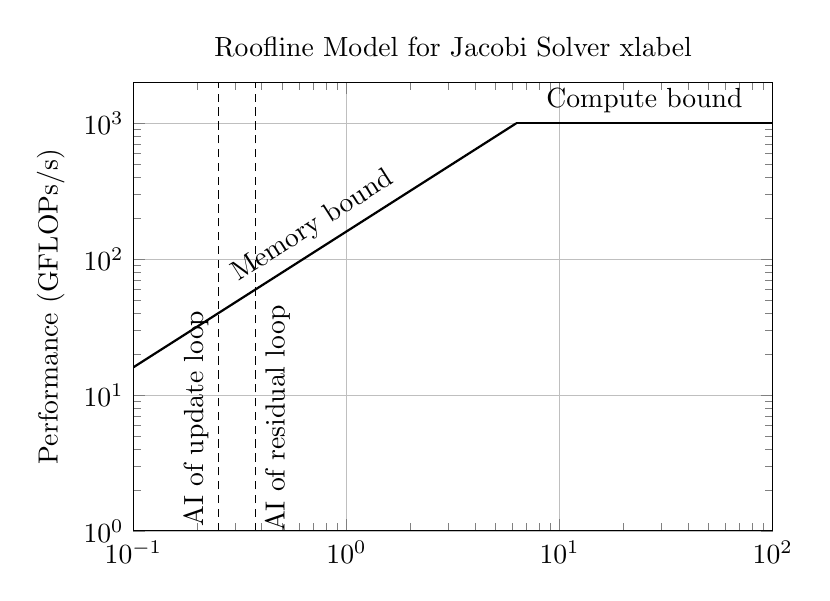
\begin{tikzpicture}
        \begin{axis}[
            title={Roofline Model for Jacobi Solver}
            xlabel={Arithmetic Intensity (FLOPs/Byte)},
            ylabel={Performance (GFLOPs/s)},
            xmode=log,
            ymode=log,
            xmin=0.1, xmax=100,
            ymin=1, ymax=2000,
            grid=major,
            major grid style={line width=.2pt,draw=gray!50},
            width=0.8\linewidth,
            height=0.6\linewidth,
        ]

        % Parameters
        \def\bandwidth{160} % Memory bandwidth in GB/s
        \def\compute{1000}  % Peak performance in GFLOPs/s
        \def\cpuai{\compute/\bandwidth} % CPU arithmetic intensity

        % Memory bound line
        \addplot [thick, domain=0.1:{\cpuai}] {\bandwidth * x}
            node[pos=0.5, above, sloped] {Memory bound};

        % Compute bound line
        \addplot [thick, domain={\cpuai}:100] {\compute}
            node[pos=0.5, above] {Compute bound};

        % Operation points
        \addplot[densely dashed] coordinates {(0.25,1) (0.25,2000)}
            node[pos=0.25, sloped, above] {AI of update loop};

        \addplot[densely dashed] coordinates {(0.375,1) (0.375,2000)}
            node[pos=0.25, sloped, below] {AI of residual loop};

        \end{axis}
    \end{tikzpicture}
\end{figure}

\end{document}